% Supplement slides for Chinese reproduction with Qwen3-4B.
% Compiler: pdflatex

\documentclass[aspectratio=169,10pt]{beamer}

\usetheme{default}
\setbeamertemplate{navigation symbols}{}
\setbeamertemplate{footline}[frame number]
\setbeamertemplate{blocks}[default]

\usepackage[T1]{fontenc}
\usepackage{lmodern}
\usepackage{booktabs}
\usepackage{tabularx}
\usepackage{array}
\usepackage{graphicx}
\usepackage{xcolor}

\graphicspath{{images/}}

\definecolor{mainblue}{RGB}{28,78,122}
\definecolor{accentred}{RGB}{178,54,48}
\definecolor{accentgreen}{RGB}{27,120,55}

\setbeamercolor{frametitle}{fg=black,bg=white}
\setbeamerfont{frametitle}{series=\bfseries,size=\large}
\setbeamercolor{title}{fg=black}
\setbeamercolor{structure}{fg=mainblue}
\setbeamercolor{block title}{fg=black,bg=gray!12}
\setbeamercolor{block body}{fg=black,bg=white}

\newcommand{\good}[1]{\textcolor{mainblue}{\textbf{#1}}}
\newcommand{\warn}[1]{\textcolor{accentred}{\textbf{#1}}}
\newcommand{\markgreen}[1]{\textcolor{accentgreen}{\textbf{#1}}}

\title{Chinese Reproduction: Qwen3-4B Addendum}
\author{C-Eval + FUR}
\date{}

\begin{document}

\subsection{Chinese Reproduction}

\begin{frame}{Chinese Reproduction: Added Qwen3-4B Runs}
\small
\begin{columns}[T,onlytextwidth]
  \begin{column}{0.48\textwidth}
    \textbf{Same FUR setting}

    \vspace{0.3em}
    \begin{tabularx}{\linewidth}{p{0.42\linewidth}>{\raggedright\arraybackslash}X}
      \toprule
      Dataset & Chinese C-Eval subset \\
      Unlearning & NPO-KL, stepwise \\
      LR / seed & \(10^{-5}\) / 1001 \\
      Specificity split & 20 held-out samples \\
      Updated params & FF2 only \\
      CoT style & Visible Chinese CoT, no thinking mode \\
      \bottomrule
    \end{tabularx}
  \end{column}

  \begin{column}{0.48\textwidth}
    \textbf{Runs compared}

    \vspace{0.3em}
    \begin{tabularx}{\linewidth}{X r r r}
      \toprule
      Run & CoTs & Targets & Epochs \\
      \midrule
      Qwen3-8B & 250 & 230 & 5 \\
      Qwen3-4B & 250 & 230 & 5 \\
      Qwen3-4B & 220 & 200 & \markgreen{10} \\
      \bottomrule
    \end{tabularx}

    \vspace{0.8em}
    \textbf{Important.}
    The \(n=220\) Qwen3-4B run is not a direct duplicate:
    it uses \markgreen{10 unlearning epochs}. We treat it as an intervention-strength
    extension, not as a pure model-size comparison.
  \end{column}
\end{columns}
\end{frame}

\begin{frame}{Three-Run Results: Matched Five-Epoch View}
\small
\begin{columns}[T,onlytextwidth]
  \begin{column}{0.54\textwidth}
    \centering
    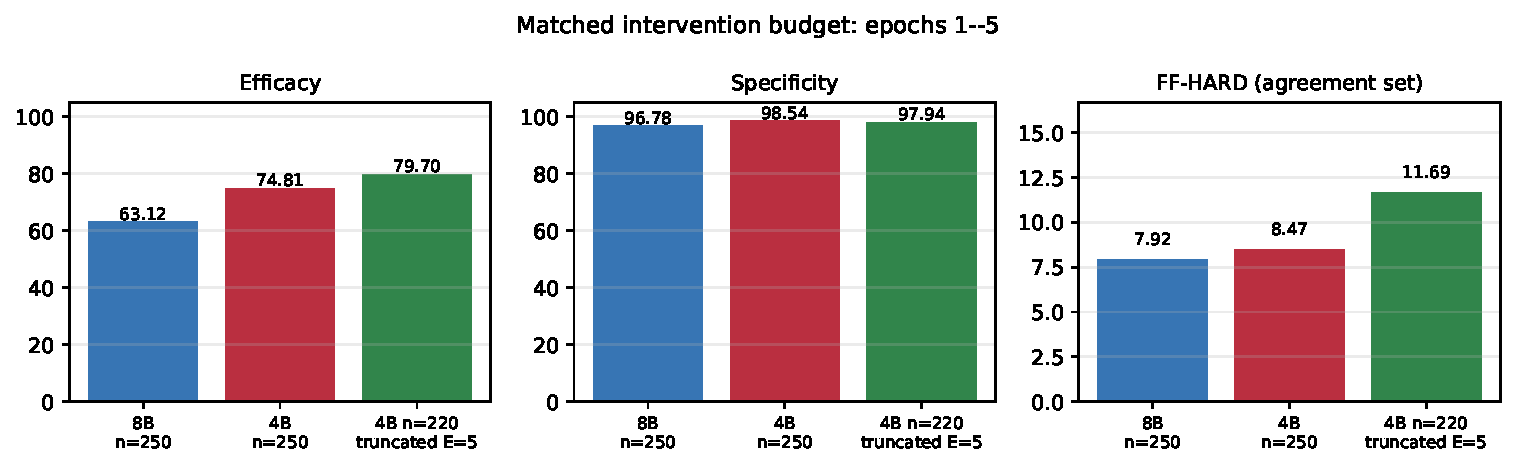
\includegraphics[width=\linewidth,height=0.76\textheight,keepaspectratio]{standard_five_epoch_comparison.pdf}
  \end{column}

  \begin{column}{0.44\textwidth}
    \textbf{Paper-style metrics through epoch 5}

    \vspace{0.3em}
    \scriptsize
    \begin{tabularx}{\linewidth}{X r r r}
      \toprule
      Run & Eff & Spec & FF-HARD \\
      \midrule
      8B, \(n=250\) & 63.12 & 96.78 & 7.92\% \\
      4B, \(n=250\) & \warn{74.81} & \good{98.54} & 8.47\% \\
      4B, \(n=220\), E5 cut & \markgreen{79.70} & 97.94 & \markgreen{11.69\%} \\
      \bottomrule
    \end{tabularx}

    \vspace{0.7em}
    \normalsize
    Under the matched \(n=250, E=5\) setting, Qwen3-4B has much higher
    efficacy than Qwen3-8B, but only a small FF-HARD gain.

    \vspace{0.5em}
    On the common eligible subset (158 questions), FF-HARD is
    \(7.59\%\) for 4B vs. \(6.96\%\) for 8B. The strongest signal is
    \good{intervention strength}, not a large faithfulness gap.
  \end{column}
\end{columns}
\end{frame}

\begin{frame}{Extended 4B Run: Epoch Effect and Probability Shifts}
\small
\begin{columns}[T,onlytextwidth]
  \begin{column}{0.50\textwidth}
    \centering
    \textbf{Unlearning trajectories}

    \vspace{0.3em}
    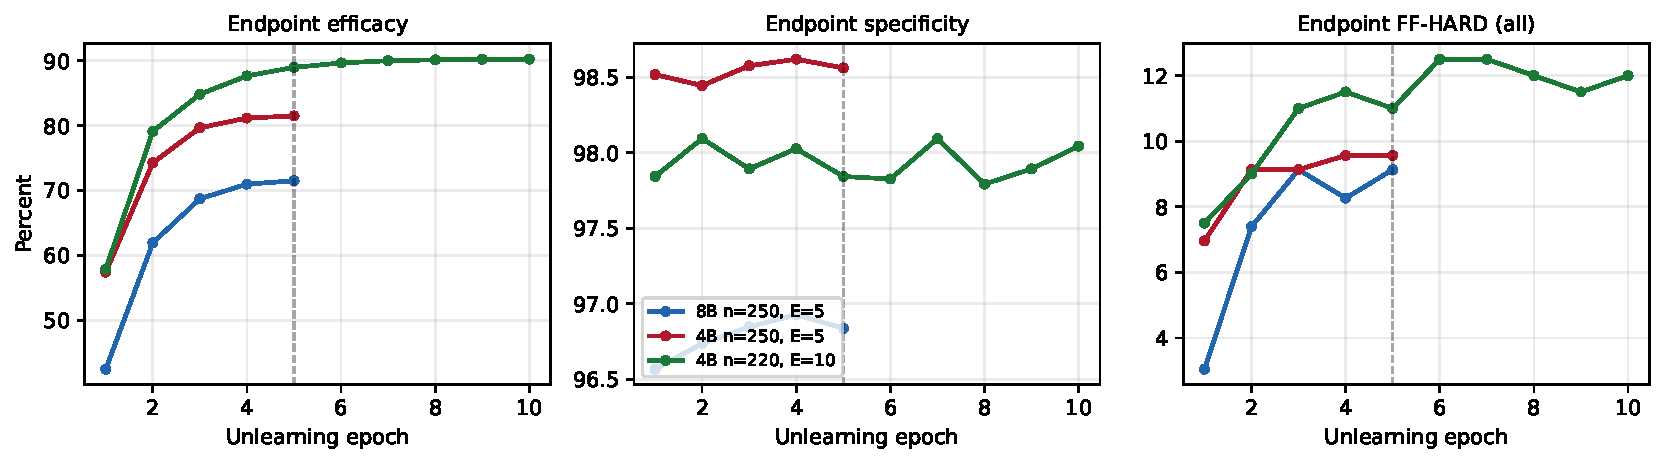
\includegraphics[width=\linewidth,height=0.55\textheight,keepaspectratio]{epoch_trajectories.pdf}

    \vspace{0.3em}
    \scriptsize
    E5 \(\rightarrow\) E10 for 4B \(n=220\):
    Eff \(88.99 \rightarrow 90.25\), FF-HARD(all) \(11.00\% \rightarrow 12.00\%\).
  \end{column}

  \begin{column}{0.50\textwidth}
    \centering
    \textbf{Endpoint FF-SOFT distribution}

    \vspace{0.3em}
    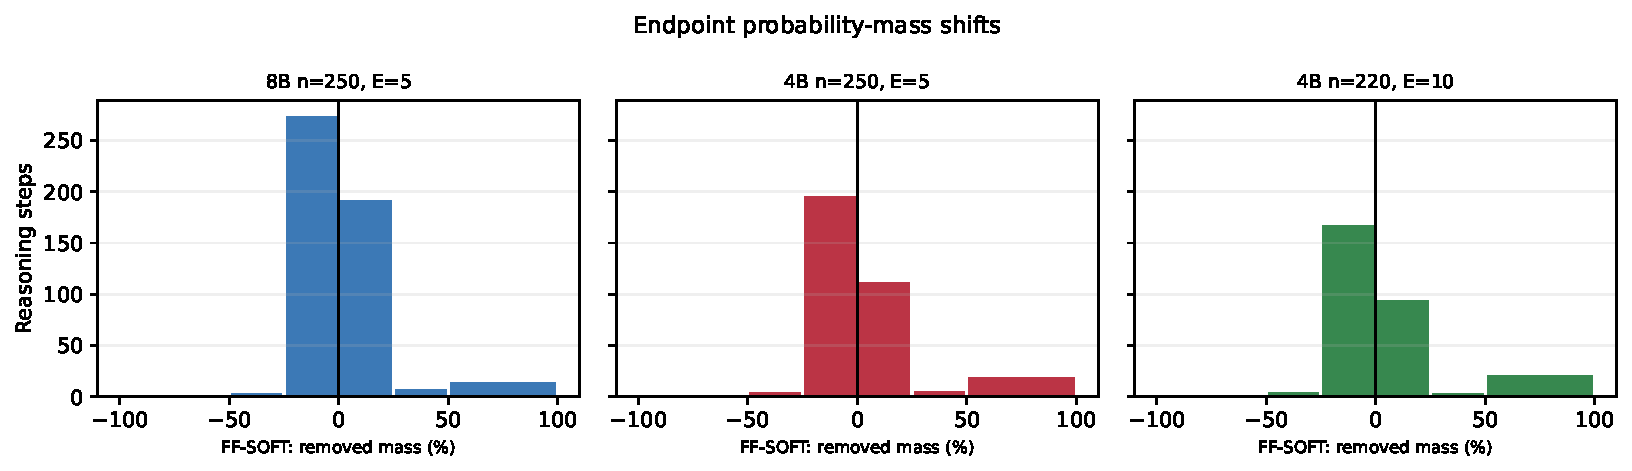
\includegraphics[width=\linewidth,height=0.55\textheight,keepaspectratio]{soft_shift_histograms.pdf}

    \vspace{0.3em}
    \scriptsize
    Ten epochs move more probability mass away from the original answer,
    but the gain saturates after roughly epoch 6.
  \end{column}
\end{columns}

\vspace{0.5em}
\textbf{Takeaway.}
\markgreen{Qwen3-4B \(n=220,E=10\) is an epoch-strength extension.}
It supports stronger intervention effects, but should not be merged into the
standard \(E=5\) model ranking.
\end{frame}

\end{document}
